\section{Empirical analysis}
We use the U.S. stock-level data of Jensen, Kelly, and Pedersen (2023).
Inspired by Section 2.5 of Didisheim, Ke, Kelly, and Malamud (2024), we retain
130 of the 153 characteristics by coverage using only the initial training
sample, 1963--1972. Validation and test observations cannot affect selection.
The published candidate dictionary is a fixed retrospective research specification;
we do not claim a historical data vintage or contemporaneous signal discovery.
We retain common stocks on the main U.S. exchanges, excluding nano stocks,
apply the 30\% row-missingness threshold, and exclude stock-months with missing
JKP next-month excess returns before monthly ranking and the calculation of $N_t$.
This complete-case convention is our sample choice, not a rule attributed to
Didisheim et al.; the sample is conditional on future payoff availability.
We rank observed characteristics into $[-0.5,0.5]$ and assign residual missing
characteristics neutral zero. We do not impute missing payoffs.

Training expands from 1963, with the preceding five formation years reserved
for validation and annual refits at the January formation close. The experiment
contains 47 test years and 564 formation months, January 1978--December 2024;
realized payoffs run from February 1978 to January 2025. Ridge penalties are
selected using the portfolio criterion introduced earlier, along 120-point grids
fixed using only the initial 1963--1972 managed-payoff spectra.

Linear is the finite-dimensional benchmark. Gaussian represents smooth nonlinear
policies; Mat\'ern-3/2 permits a broader nonlinear class. Each nonlinear policy
uses one fixed map of 10,000 random Fourier features, seed zero. Both share
a lengthscale of 4.3921, the median distance among 1,000 initial-training vectors.
A common fixed positive scale targets median gross exposure 1.8 for the initial
Linear validation policy. The last validation payoff becomes known at the
January 1978 formation close, before the first OOS payoff.

Figure~\ref{fig:wealth} and Table~\ref{tab:performance} summarize the new run.
Linear: Sharpe 3.09, maximum drawdown -15.8\%; Gaussian: Sharpe 3.30, maximum drawdown -15.6\%; Mat\'ern-3/2: Sharpe 3.46, maximum drawdown -13.6\%.
Total wealth compounds the cash return plus the scaled portfolio excess payoff,
adding cash exactly once. Drawdown uses exactly that wealth path, including
its starting value.
\begin{figure}[htbp]\centering
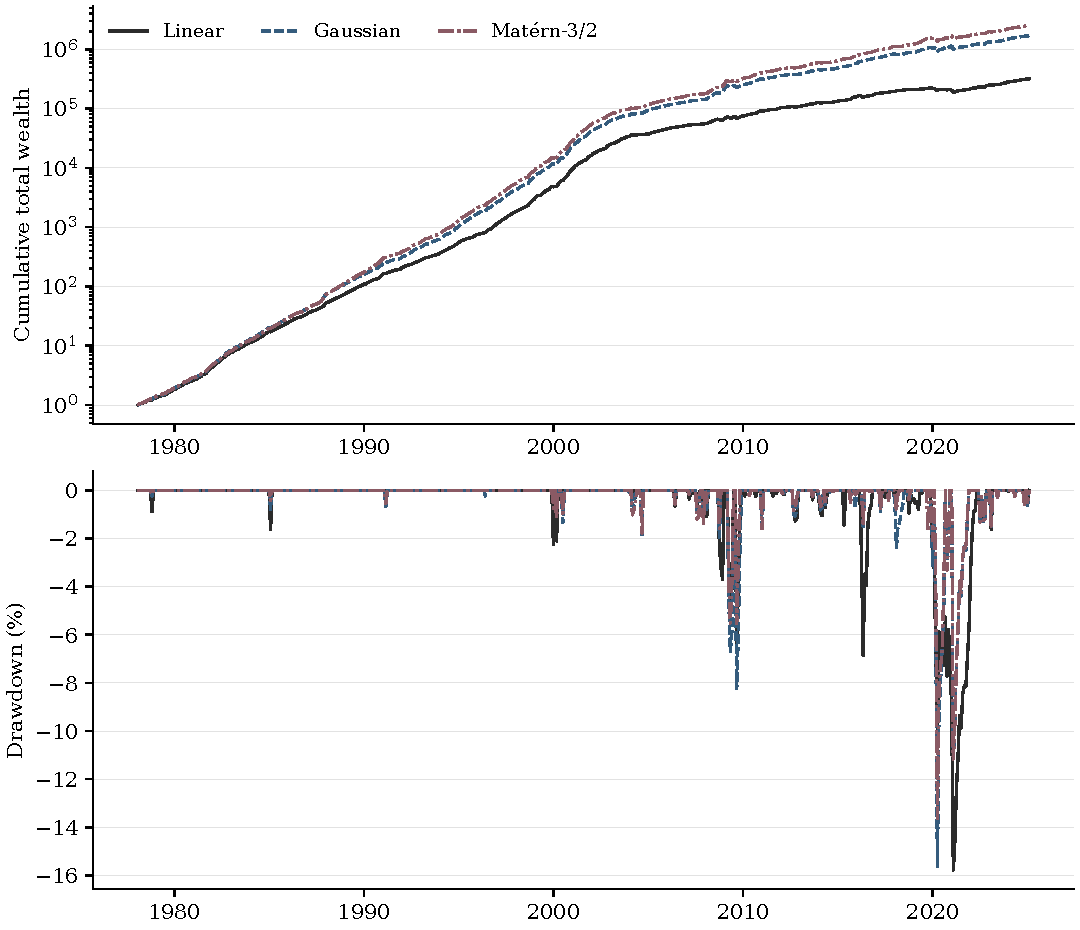
\includegraphics[width=.9\linewidth]{figures/fig01_wealth_drawdown.pdf}
\caption{Cumulative total wealth (log scale) and drawdown from the same wealth series.
All policies use the same fixed pre-payoff scale.}\label{fig:wealth}
\end{figure}
\begin{table}[htbp]\centering\small
\resizebox{\linewidth}{!}{\begin{tabular}{lrrrrrr}
\toprule
Policy & Annual mean excess & Annual vol. & Sharpe & Max. drawdown & Mean gross & Mean net \\
\midrule
Linear & 0.234 & 0.076 & 3.091 & -0.158 & 2.009 & 0.132 \\
Gaussian & 0.272 & 0.082 & 3.300 & -0.156 & 2.326 & 0.100 \\
Matérn-3/2 & 0.280 & 0.081 & 3.461 & -0.136 & 2.374 & 0.090 \\
\bottomrule
\end{tabular}
}
\caption{Performance from the 564 monthly OOS observations. Returns and volatility
are annualized from decimal monthly excess returns; maximum drawdown is signed.}
\label{tab:performance}\end{table}

Figure~\ref{fig:exposure} reports gross and net stock exposure under the same scale.
\begin{figure}[htbp]\centering
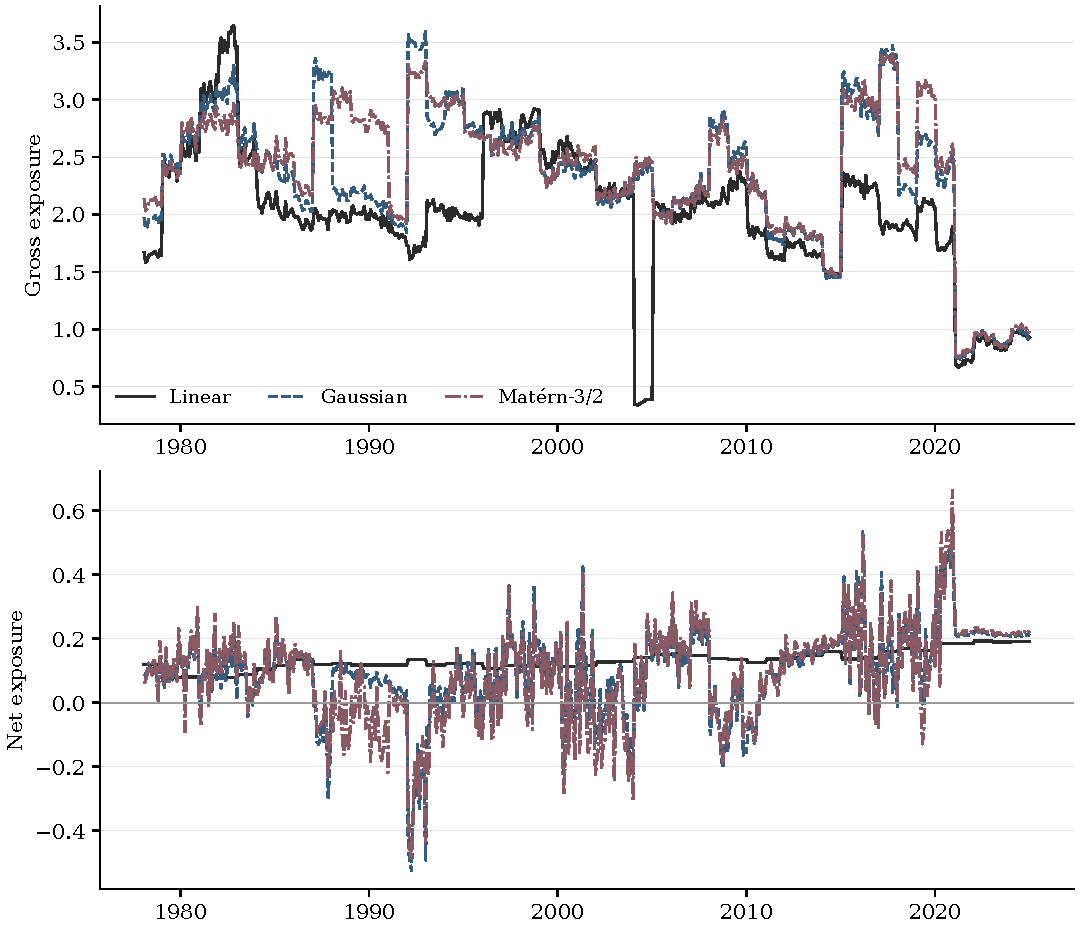
\includegraphics[width=.9\linewidth]{figures/fig02_exposure.pdf}
\caption{Gross and net exposures for the three policies.}\label{fig:exposure}
\end{figure}

Representation determines which investment opportunities can potentially be
expressed. The managed-portfolio spectrum describes their payoff structure.
Effective complexity determines how much of that spectrum is actually used
after regularization. Figure~\ref{fig:spectrum} shows the ordered positive
second-moment eigenvalues on the common history preceding the 2024 test window.
\begin{figure}[htbp]\centering
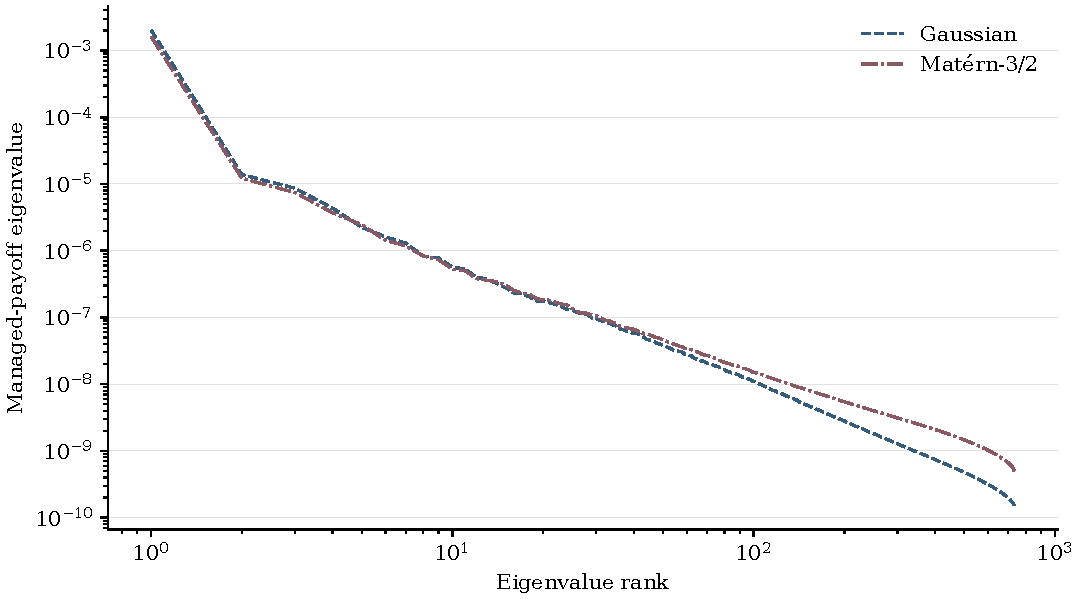
\includegraphics[width=.9\linewidth]{figures/fig05_managed_spectrum.pdf}
\caption{Managed-portfolio spectra on log-log axes.}\label{fig:spectrum}
\end{figure}

Figures~\ref{fig:gaussian} and~\ref{fig:matern} plot historical and subsequent
2024 test Sharpe against $C(\lambda)=\sum_j\mu_j/(\mu_j+\lambda)$ along the
same frozen penalty paths. The test panels use only the twelve payoffs from
February 2024 through January 2025. Validation selections are distinguished
from descriptive ex-post maxima, which never determine the policy.
\begin{figure}[htbp]\centering
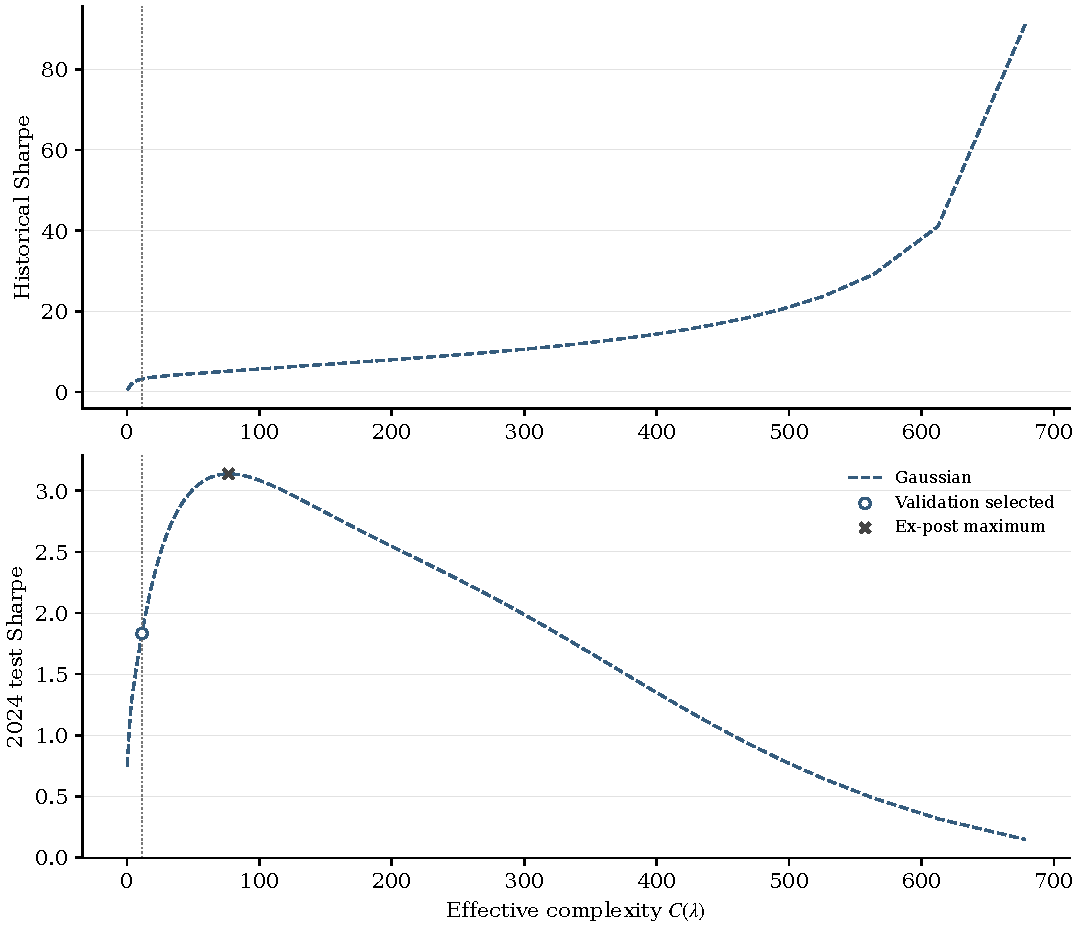
\includegraphics[width=.9\linewidth]{figures/fig03_complexity_gaussian.pdf}
\caption{Gaussian effective complexity: historical and true 2024 test Sharpe.}
\label{fig:gaussian}\end{figure}
\begin{figure}[htbp]\centering
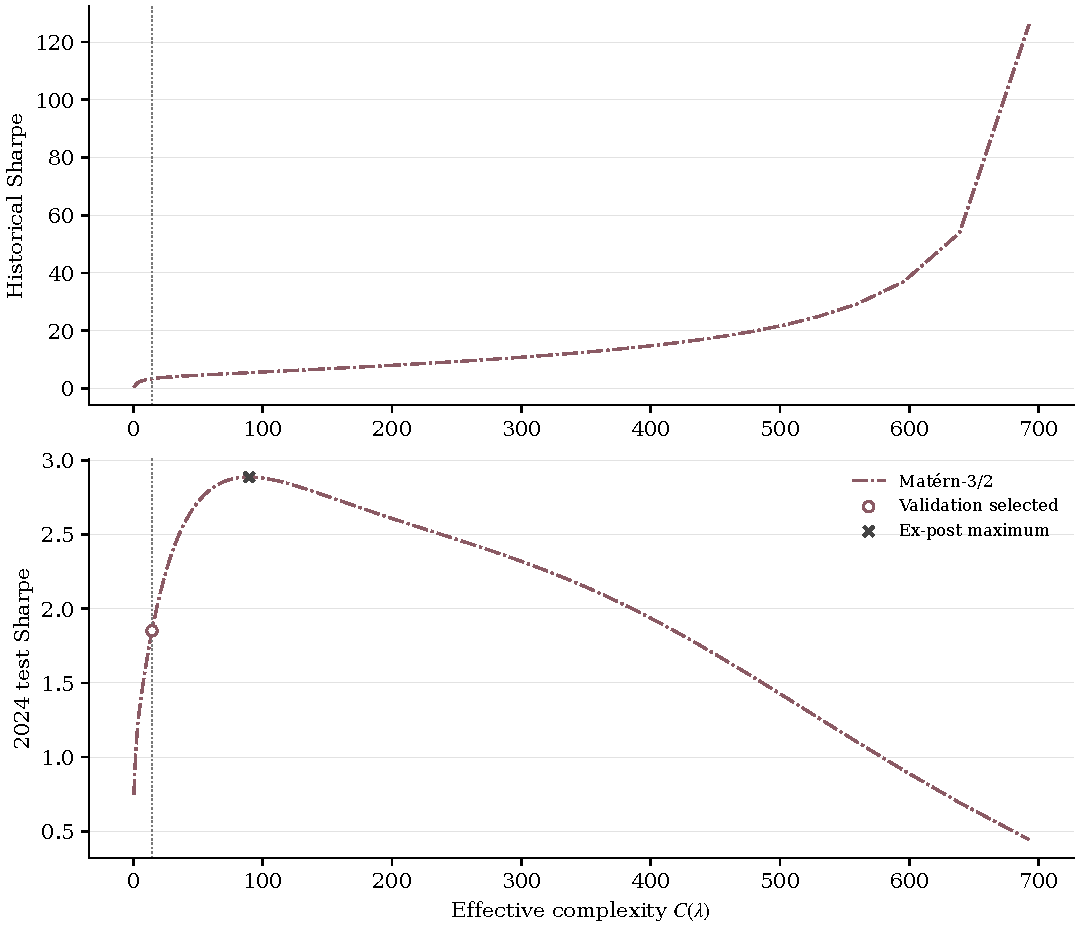
\includegraphics[width=.9\linewidth]{figures/fig04_complexity_matern32.pdf}
\caption{Mat\'ern-3/2 effective complexity: historical and true 2024 test Sharpe.}
\label{fig:matern}\end{figure}
